\documentclass[10pt,letterpaper]{article}
\usepackage[margin=1in]{geometry}
\usepackage{amsmath,amssymb,amsthm,mathtools}
\usepackage{graphicx}
\usepackage{booktabs}
\usepackage[numbers,sort&compress]{natbib}
\usepackage[hidelinks]{hyperref}
\usepackage{xcolor}
\usepackage{microtype}
\usepackage{caption}
\captionsetup{font=small,labelfont=bf}
\newtheorem{theorem}{Theorem}
\newtheorem{lemma}{Lemma}
\newtheorem{proposition}{Proposition}
\newtheorem{corollary}{Corollary}
\theoremstyle{definition}
\newtheorem{definition}{Definition}
\newcommand{\SB}{\Sigma^{\mathrm{B}}}
\newcommand{\SW}{\Sigma^{\mathrm{W}}}
\newcommand{\Deff}{D_{\mathrm{eff}}}
\newcommand{\LCPFDRDeight}{0.876\,(0.015)}
\newcommand{\LCPpowDeight}{0.005}
\newcommand{\BOUNDpowDeight}{0.000}
\newcommand{\ORACLEpowDeight}{0.000}
\newcommand{\MCpowDeight}{0.000}
\newcommand{\LCPFDRDtwelve}{0.246\,(0.028)}
\newcommand{\LCPpowDtwelve}{0.003}
\newcommand{\BOUNDpowDtwelve}{0.003}
\newcommand{\ORACLEpowDtwelve}{0.054}
\newcommand{\MCpowDtwelve}{0.000}
\newcommand{\LCPFDRDsixteen}{0.089\,(0.017)}
\newcommand{\LCPpowDsixteen}{0.015}
\newcommand{\BOUNDpowDsixteen}{0.016}
\newcommand{\ORACLEpowDsixteen}{0.210}
\newcommand{\MCpowDsixteen}{0.000}
\newcommand{\LCPFDRDtwentyfour}{0.046\,(0.006)}
\newcommand{\LCPpowDtwentyfour}{0.105}
\newcommand{\BOUNDpowDtwentyfour}{0.108}
\newcommand{\ORACLEpowDtwentyfour}{0.531}
\newcommand{\MCpowDtwentyfour}{0.000}
\newcommand{\LCPFDRDforty}{0.050\,(0.002)}
\newcommand{\LCPpowDforty}{0.463}
\newcommand{\BOUNDpowDforty}{0.458}
\newcommand{\ORACLEpowDforty}{0.851}
\newcommand{\MCpowDforty}{0.010}
\newcommand{\PBFDRrange}{0.13--0.14}
\newcommand{\OtherFDRrange}{0.08--0.13}
\newcommand{\QQLCP}{0.072--0.077}
\newcommand{\QQORACLE}{0.090--0.112}
\newcommand{\STRESSLCPFDR}{0.224\,(0.024)}
\newcommand{\STRESSPBFDR}{0.247}
\newcommand{\PBSSmax}{0.22}
\newcommand{\SEAADnsForty}{0.98}
\newcommand{\LEEnsForty}{0.69}
\newcommand{\DeffSEAADcap}{0.53}
\newcommand{\DeffLEEcap}{0.53}
\newcommand{\DeffSEAADfull}{0.90}
\newcommand{\DeffLEEfull}{0.98}
\newcommand{\RealG}{417}
\newcommand{\RealPairs}{86{,}736}
\newcommand{\SEAADfullLCP}{34{,}944}
\newcommand{\SEAADfullPB}{36{,}715}
\newcommand{\SEAADfullMC}{28{,}364}
\newcommand{\SEAADfullLCPfrac}{0.40}
\newcommand{\SEAADleakFull}{0.004}
\newcommand{\SEAADleakCap}{0.026}
\newcommand{\LEEfullLCP}{42{,}075}
\newcommand{\LEEfullPB}{44{,}951}
\newcommand{\LEEfullMC}{36{,}270}
\newcommand{\LEEfullLCPfrac}{0.49}
\newcommand{\LEEleakFull}{0.002}
\newcommand{\LEEleakCap}{0.081}
\newcommand{\precLCPDtwentyfour}{0.94}
\newcommand{\recLCPDtwentyfour}{0.32}
\newcommand{\precPBDtwentyfour}{0.92}
\newcommand{\recPBDtwentyfour}{0.39}
\newcommand{\precMCDtwentyfour}{1.00}
\newcommand{\recMCDtwentyfour}{0.01}
\newcommand{\precLCPDforty}{0.94}
\newcommand{\recLCPDforty}{0.55}
\newcommand{\precPBDforty}{0.92}
\newcommand{\recPBDforty}{0.60}
\newcommand{\precMCDforty}{0.97}
\newcommand{\recMCDforty}{0.28}
\newcommand{\capNwithin}{93 (SEA-AD) and 33 (Lee)}
\newcommand{\capLCPSEAAD}{0.025}
\newcommand{\capPBSEAAD}{0.075}
\newcommand{\capnaiveSEAAD}{0.086}
\newcommand{\capMCSEAAD}{0.004}
\newcommand{\SEAADleakSplit}{0.024}
\newcommand{\capLCPLEE}{0.020}
\newcommand{\capPBLEE}{0.020}
\newcommand{\capnaiveLEE}{0.020}
\newcommand{\capMCLEE}{0.020}
\newcommand{\LEEleakSplit}{0.086}
\newcommand{\xLCPbyPB}{0.60}
\newcommand{\xPBbyLCP}{0.57}
\newcommand{\replLCP}{0.58}
\newcommand{\rhoLCP}{0.60}
\newcommand{\replPB}{0.60}
\newcommand{\rhoPB}{0.61}
\newcommand{\replPBonly}{0.38}
\newcommand{\nPBonly}{4{,}039}
\newcommand{\sexRhoRange}{-0.95 to -0.60}
\newcommand{\sexWithinMax}{0.09}
\newcommand{\hsRhoSEAAD}{0.82}
\newcommand{\hsWSEAAD}{0.30}
\newcommand{\hsLCPSEAAD}{0.98}
\newcommand{\hsRhoLEE}{0.78}
\newcommand{\hsWLEE}{0.42}
\newcommand{\hsLCPLEE}{1.00}
\newcommand{\HOn}{5}
\newcommand{\HOLCPFDRrange}{0.041--0.050}
\newcommand{\HOratio}{0.89--1.04}
\newcommand{\HOPBFDRrange}{0.08--0.30}
\newcommand{\HOsixteenFDR}{0.040\,(0.005)}
\newcommand{\HELDOUTsentence}{With a new gene panel, new seeds and three designs built from real donors' cell numbers and depths, the frozen validity criterion held in all 5 held-out designs with at least 24 donors: LCP's FDR was 0.041--0.050 and its power 0.89--1.04 times BOUND's, while pseudobulk's FDR was 0.08--0.30. With 16 donors but about 100 cells each, LCP's FDR was 0.040\,(0.005) (pseudobulk 0.13), so the 16-donor failure in development depends on cells per donor as well as on the number of donors.}
\newcommand{\ABLCPgpuFsixteen}{0.083}
\newcommand{\ABLCPgpuPsixteen}{0.014}
\newcommand{\ABLCPgpuSsixteen}{0.048}
\newcommand{\ABLCPnoleakFsixteen}{0.045}
\newcommand{\ABLCPnoleakPsixteen}{0.017}
\newcommand{\ABLCPnoleakSsixteen}{0.108}
\newcommand{\ABLCPtruevFsixteen}{0.075}
\newcommand{\ABLCPtruevPsixteen}{0.017}
\newcommand{\ABLCPtruevSsixteen}{0.056}
\newcommand{\ABLCPunstdFsixteen}{0.346}
\newcommand{\ABLCPunstdPsixteen}{0.023}
\newcommand{\ABLCPunstdSsixteen}{0.093}
\newcommand{\ABPBpermFsixteen}{0.068}
\newcommand{\ABPBpermPsixteen}{0.015}
\newcommand{\ABPBpermSsixteen}{0.121}
\newcommand{\ABLCPgpuFtwentyfour}{0.046}
\newcommand{\ABLCPgpuPtwentyfour}{0.107}
\newcommand{\ABLCPgpuStwentyfour}{0.054}
\newcommand{\ABLCPnoleakFtwentyfour}{0.043}
\newcommand{\ABLCPnoleakPtwentyfour}{0.123}
\newcommand{\ABLCPnoleakStwentyfour}{0.141}
\newcommand{\ABLCPtruevFtwentyfour}{0.049}
\newcommand{\ABLCPtruevPtwentyfour}{0.112}
\newcommand{\ABLCPtruevStwentyfour}{0.056}
\newcommand{\ABLCPunstdFtwentyfour}{0.148}
\newcommand{\ABLCPunstdPtwentyfour}{0.096}
\newcommand{\ABLCPunstdStwentyfour}{0.099}
\newcommand{\ABPBpermFtwentyfour}{0.074}
\newcommand{\ABPBpermPtwentyfour}{0.115}
\newcommand{\ABPBpermStwentyfour}{0.160}
\newcommand{\ABLCPgpuFforty}{0.049}
\newcommand{\ABLCPgpuPforty}{0.470}
\newcommand{\ABLCPgpuSforty}{0.051}
\newcommand{\ABLCPnoleakFforty}{0.058}
\newcommand{\ABLCPnoleakPforty}{0.495}
\newcommand{\ABLCPnoleakSforty}{0.214}
\newcommand{\ABLCPtruevFforty}{0.050}
\newcommand{\ABLCPtruevPforty}{0.460}
\newcommand{\ABLCPtruevSforty}{0.056}
\newcommand{\ABLCPunstdFforty}{0.101}
\newcommand{\ABLCPunstdPforty}{0.381}
\newcommand{\ABLCPunstdSforty}{0.098}
\newcommand{\ABPBpermFforty}{0.087}
\newcommand{\ABPBpermPforty}{0.462}
\newcommand{\ABPBpermSforty}{0.223}


\title{Between-donor gene co-expression from few donors:\\ a leak-corrected permutation test and a bound on what any test can detect}
\author{[Author names and affiliations to be added by the authors]}
\date{}

\begin{document}
\maketitle

\begin{abstract}
In multi-donor single-cell RNA-seq, two genes can co-vary within donors, reflecting cell-state programs, or between donors, reflecting donor-level variation such as genotype, environment or disease. Between-donor co-expression is usually tested by correlating pseudobulk donor means. We show that this targets a different quantity. With cells sampled independently within donors, the covariance of donor ratio-means equals the between-donor covariance plus the within-donor covariance scaled by each donor's effective inverse cell count, so cell-state programs leak into pseudobulk and are reported as donor-level associations when donors contribute few cells. We give an unbiased count-scale correction for this leak, estimated from each donor's own cells, and prove an information bound for testing one gene pair under a Gaussian working model: with D donors, no test has more local power than an oracle that observes the true donor means of only $D_{\mathrm{eff}}=\sum_d\rho_{dj}\rho_{dk}$ donors, where $\rho$ is the donor-specific reliability of a donor mean. At about 40 cells per donor, $D_{\mathrm{eff}}$ is roughly a quarter to a half of D for typical genes in two Alzheimer's disease microglia cohorts, which quantifies why few-donor, few-cell designs cannot resolve pair-level between-donor structure. We propose LCP, a leak-corrected, precision-standardized donor-permutation test. In simulations with exact ground truth, LCP controls the false discovery rate from 24 donors upward and matches the power of a noise-limited oracle benchmark, whereas pseudobulk correlation has a false discovery rate of 0.13--0.14 at 24--40 donors and a moment-corrected test with a donor jackknife has almost no power. In five frozen held-out designs with 24--40 donors, three of them built from real donors' cell numbers and sequencing depths, LCP's false discovery rate was 0.041--0.050, at 0.89--1.04 times the power of the noise-limited benchmark, while pseudobulk's was 0.08--0.30. We also report negative results: at 16 or fewer donors with about 40 cells each, no test based on observed donor means, ours included, is calibrated in the tail used for multiple-testing correction (with 100 cells per donor, LCP was calibrated at 16 donors in a held-out design); LCP is not protected when sequencing depth is coupled to cell state; and covariance intervals undercover even when computed from the true donor means. In SEA-AD (84 donors) and Lee et al. 2026 (80 donors) microglia, the leak is under 1\% of the pseudobulk covariance at the cohorts' real cell numbers, and LCP and pseudobulk largely agree; when donors are reduced to 40 cells the leak grows to 2--9\%. Code: \url{https://github.com/kaapra081/fewdonor-coexpression}.

\end{abstract}

\section{Introduction}

Multi-donor single-cell RNA-seq cohorts now profile tens to hundreds of donors per cell type, and gene--gene co-expression is computed in them routinely, for network inference, module discovery and co-expression QTL mapping \citep{Li2023coeQTL}. Two genes can co-vary for two different reasons. They can co-vary \emph{within} donors, across the cells of one person, as members of a cell-state program; or they can co-vary \emph{between} donors, because donor-level factors (genotype, sex, age, disease, post-mortem handling) shift both genes' mean expression together. The two levels answer different biological questions, and a pooled analysis of all cells mixes them.

The between-donor level is usually studied with pseudobulk: average each donor's cells, then correlate the donor means across donors. Pseudobulk has become the default for donor-level single-cell inference because it respects the donor as the unit of replication \citep{Squair2021,Zimmerman2021}. For co-expression it has a less obvious problem. A donor mean computed from $n_d$ cells carries finite-cell sampling error, and when two genes co-vary within donors their sampling errors co-vary as well. This within-donor covariance \emph{leaks} into the covariance of donor means and is reported as donor-level association. The leak is largest when it matters most: in rare cell types and small cohorts, where donors contribute tens rather than hundreds of cells.

We study the between-donor covariance $\SB$ of latent expression on the count scale and make four contributions.
(i) We derive the leak exactly under a Poisson measurement model (Lemma~\ref{lem:leak}): pseudobulk covariance targets $\SB+\bar\kappa\,\SW$, where $\bar\kappa\approx\overline{1/n_d}$, and the leak can be estimated without bias from each donor's own cells.
(ii) We prove an information bound for testing a single gene pair (Theorem~\ref{thm:bound}): with $D$ donors, no test has more local power than an oracle that observes the true donor means of $\Deff=\sum_d\rho_{dj}\rho_{dk}$ donors, where $\rho_{dj}$ is the reliability of donor $d$'s mean for gene $j$. At about 40 cells per donor, $\Deff$ is between a quarter and a half of $D$ for typical genes in the two cohorts we analyse. This gives a design rule (donors are worth far more than cells) and an honest yardstick for any method.
(iii) We propose LCP, a leak-corrected, precision-standardized donor-permutation test, give a proof outline that it is asymptotically exact under the null of independent donor effects, and show that its efficiency relative to the bound depends only on the spread of donor reliabilities (Theorem~\ref{thm:lcp}, Proposition~\ref{prop:are}).
(iv) We report, with exact-truth simulations and frozen held-out designs that use the real cell numbers and sequencing depths of two Alzheimer's disease microglia cohorts, where LCP works and where nothing does: LCP controls the false discovery rate (FDR) from 24 donors upward and matches the power of a noise-limited oracle, whereas pseudobulk correlation inflates the FDR to \PBFDRrange{} and the existing moment-corrected test has almost no power; at 16 or fewer donors no test based on observed donor means, ours included, is calibrated in the tail that multiple-testing correction uses, and covariance intervals undercover even when computed from the true donor means.

\paragraph{Related work.}
The moment correction that subtracts a known, heteroscedastic, correlated error covariance from an observed covariance is classical: it is the BCES estimator of astronomy \citep{AkritasBershady1996,Kelly2007}, and precision-weighted debiased versions are used in Mendelian randomization \citep{Ye2021dIVW} and cross-trait LD score regression \citep{BulikSullivan2015b}. Multivariate random-effects meta-analysis treats study-level estimates with known within-study covariance \citep{JacksonWhiteRiley2013,RileyAbramsSutton2007}, and multilevel covariance-structure models separate within- and between-group covariance \citep{Muthen1994,Ludtke2008}. Attenuation of correlations by measurement error goes back to Spearman \citep{Fuller1987}. Single-cell methods estimate within-donor co-expression with measurement-error models (CS-CORE \citep{Su2023CSCORE}, memento \citep{Kim2024memento}, SPLN \citep{GeLi2026SPLN}), and co-expression QTL methods target between-donor variation \citep{Li2023coeQTL}; none provides a count-scale leak correction or a calibrated few-donor test for $\SB$. Our contribution is not the moment correction itself but the count-derived per-donor leak, the per-pair information bound, a test that attains it, and an explicit map of the regime in which between-donor co-expression cannot be resolved.

\section{Setting and estimand}

Donors $d=1,\dots,D$ contribute $n_d$ cells of one type. Cell $i$ has latent relative expression $\theta_i\in\mathbb{R}^G_+$ (expected UMI count per unit library size) and library size $s_i$; counts are $Y_{ij}\mid\theta_i,s_i\sim\mathrm{Poisson}(s_i\theta_{ij})$, independently across genes (extra-Poisson noise independent across genes is absorbed into $\theta$). Donor $d$'s cells are i.i.d.\ from a donor-specific distribution $F_d$, and the $F_d$ are i.i.d.\ draws from a donor population; the design ($n_d$ and the $s_i$) is ancillary and may differ arbitrarily between donors. With $\mu_{dj}=\mathrm{E}_{F_d}[\theta_j]$, the estimands are
\[
\SB_{jk}=\mathrm{Cov}(\mu_{dj},\mu_{dk}),\qquad \SW_{jk}=\mathrm{E}\big[\mathrm{Cov}_{F_d}(\theta_j,\theta_k)\big],
\]
with donors weighted equally. Off-diagonal entries of both are identified from count moments; the latent scale avoids the depth artefacts of log-normalized data. We test $H_0:\SB_{jk}=0$ for all pairs and control the FDR with Benjamini--Hochberg (BH).

Per donor we use the ratio mean $m_{dj}=\sum_iY_{ij}/S_d$ ($S_d=\sum_is_i$), the depth-heterogeneity factor $\kappa_d=\sum_is_i^2/S_d^2$ ($=1/n_d$ at equal depth), the sample covariance $\hat C_d$ of $x_i=Y_i/s_i$, and the sampling variance $\hat\psi_{dj}=\kappa_d\hat\sigma^2_{dj}+m_{dj}/S_d$, where $\hat\sigma^2_{dj}$ is the Poisson-corrected within-donor variance.

\section{The leak}

\begin{lemma}[Leak]\label{lem:leak}
For $j\neq k$, $\mathrm{E}[m_{dj}\mid F_d]=\mu_{dj}$ and $\mathrm{Cov}(m_{dj},m_{dk}\mid F_d)=\kappa_d\,\mathrm{Cov}_{F_d}(\theta_j,\theta_k)$. Hence $\mathrm{Cov}(m_{dj},m_{dk})=\SB_{jk}+\kappa_d\SW_{jk}$, and $\mathrm{E}[\kappa_d\hat C_{d,jk}\mid F_d]=\kappa_d\mathrm{Cov}_{F_d}(\theta_j,\theta_k)$.
\end{lemma}
The proof (Appendix~\ref{app:proofs}) uses only conditional independence of Poisson draws across genes and of cells within a donor. Two consequences follow. First, the covariance of donor means---the quantity pseudobulk correlation tests---equals $\SB+\bar\kappa\SW$; within-only programs ($\SB_{jk}=0$, $\SW_{jk}\neq0$) are called at a rate that grows with $\bar\kappa$, i.e.\ with fewer cells per donor. Second, the leak is known in form and estimable per donor, so
$\hat\SB_{jk}=S_{B,jk}-D^{-1}\sum_d\kappa_d\hat C_{d,jk}$
is unbiased for $\SB_{jk}$ (Proposition~\ref{prop:unbiased}, Appendix). With equal weights this is the BCES correction \citep{AkritasBershady1996} with a count-derived error covariance; we do not claim it as new.

\section{What any per-pair test can detect}

Write $a_d=\SB_{jj}+\psi_{dj}$, $b_d=\SB_{kk}+\psi_{dk}$ for the total variances of donor means, and $\rho_{dj}=\SB_{jj}/a_d$ for the reliability of donor $d$'s mean of gene $j$.

\begin{theorem}[Information bound]\label{thm:bound}
Let $m_d\sim N(\bar\mu,\SB+\Psi_d)$ independently with known sampling covariances $\Psi_d$, and consider $\sigma=\SB_{jk}$ with nuisance parameters $(\bar\mu,\SB_{jj},\SB_{kk})$. Donor $d$ contributes Fisher information $I_d(\sigma)=(a_db_d+c_d^2)/(a_db_d-c_d^2)^2$ with $c_d=\sigma+\ell_d$ ($\ell_d$ the leak). At $\sigma=0$ without leak the nuisance parameters are information-orthogonal to $\sigma$ and the efficient information is $I=\sum_d1/(a_db_d)$, against $I^\ast=D/(\SB_{jj}\SB_{kk})$ for an oracle that observes $\mu_d$. Consequently, for local alternatives $\sigma=h/\sqrt D$, no asymptotically level-$\alpha$ test based on genes $j$ and $k$ has power exceeding that of the oracle test with
\[
\Deff=\sum_{d=1}^D\rho_{dj}\rho_{dk}\quad\text{donors.}
\]
\end{theorem}
Theorem~\ref{thm:bound} is the per-pair, heteroscedastic form of attenuation by measurement error; its use here is quantitative. With $\psi_{dj}\approx c_j/n_d$, $\rho_{dj}=(1+c_j/(\SB_{jj}n_d))^{-1}$: doubling cells per donor at most doubles $\Deff$ and saturates at $D$, while adding donors raises $\Deff$ linearly. In SEA-AD microglia the median noise-to-signal ratio $\psi_{dj}/\SB_{jj}$ at 40 cells per donor is \SEAADnsForty{} (Lee 2026: \LEEnsForty{}), so at 16 donors and ${\sim}40$ cells the best possible per-pair test for a typical gene pair behaves like an oracle with four to five donors.

\section{LCP: a leak-corrected, precision-standardized permutation test}

For each gene, a Paule--Mandel random-effects fit to $(m_{dj},\hat\psi_{dj})_d$ gives $\hat\mu_j$ and $\hat\tau^2_j$ (an estimate of $\SB_{jj}$), solving $\sum_d(m_{dj}-\hat\mu_j)^2/(\hat\tau_j^2+\hat\psi_{dj})=D-1$. Standardize $r_{dj}=(m_{dj}-\hat\mu_j)/\hat v_{dj}^{1/2}$ with $\hat v_{dj}=\hat\tau^2_j+\hat\psi_{dj}$, and for each pair form
\[
T_{jk}=\Big[\sum_d\big(r_{dj}r_{dk}-\tilde\ell_{d,jk}\big)\Big]\sqrt{\tfrac{D}{D+\sum_d\tilde\ell_{d,jk}^2}},\qquad \tilde\ell_{d,jk}=\frac{\kappa_d\hat C_{d,jk}}{(\hat v_{dj}\hat v_{dk})^{1/2}}.
\]
The reference distribution is that of $T^\pi_{jk}=\sum_dr_{\pi(d)j}r_{dk}$ over random donor permutations $\pi$ (20{,}000, refined to $4\times10^5$ when $p\le5\times10^{-4}$); permuted pairings come from different donors and therefore carry no leak. Each choice addresses a failure we observed: the leak term removes within-only false positives; standardization by the model-based total variance equalizes heteroscedastic donors (and, because of the Paule--Mandel root, fixes $\sum_dr_{dj}^2=D-1$, so the permutation variance is deterministic); and permutation replaces normal-theory references, which at 16 donors are anti-conservative in the BH-relevant tail even for Pearson correlation of the \emph{true} donor means. All pairs share one set of permutations, so the cost is a sequence of $G\times D$ by $D\times G$ matrix products.

\begin{theorem}[Validity]\label{thm:lcp}
Let $H_0$: the donor-level vectors $(\mu_{dj})_d$ and $(\mu_{dk})_d$ are independent. (a) If the leak is absent and the standardized deviations of one gene are exchangeable across donors, the LCP $p$-value is exactly valid. (b) Under bounded designs, bounded $4+\delta$ moments and consistent per-gene nuisance estimates, $T_{jk}/\sqrt D\Rightarrow N(0,1)$ under $H_0$ as $D\to\infty$, and the permutation distribution of $T^\pi_{jk}/\sqrt D$ converges in probability to the same limit, so LCP is asymptotically exact.
\end{theorem}
\begin{proposition}[Efficiency]\label{prop:are}
Under the model of Theorem~\ref{thm:bound}, the asymptotic relative efficiency of LCP with respect to the bound is $\big[D^{-1}\sum_d(\rho_{dj}\rho_{dk})^{1/2}\big]^2/\big[D^{-1}\sum_d\rho_{dj}\rho_{dk}\big]\le1$, with equality iff $\rho_{dj}\rho_{dk}$ is constant across donors.
\end{proposition}
Proofs are in Appendix~\ref{app:proofs}; part (b) of Theorem~\ref{thm:lcp} is an outline whose finite-$D$ accuracy we assess by simulation. LCP tests independence, not the weaker $\SB_{jk}=0$: if donor effects are dependent but uncorrelated, the permutation variance is wrong (the phenomenon studentized permutation tests address \citep{DiCiccioRomano2017}). Studentizing restored weak-null validity in our development runs but removed almost all power at 16 donors, so we report the weak null as a stress case.

\section{Simulations}

\paragraph{Design.} The simulator has exact analytic truth on the latent scale and was checked numerically. Each gene panel (80 genes, 3{,}160 pairs) contains within-only programs (moderate and strong), between-only programs, programs at both levels with same and opposite signs, a sign-heterogeneous within-donor null, a between-donor weak null (dependent but uncorrelated donor effects) and independent genes. Donor effects are log-normal, with gene-specific donor variation matched to SEA-AD (median between-donor log-SD 0.19), and per-cell depths are taken from the SEA-AD fit. Development designs vary $D\in\{8,12,16,24,40\}$ with ${\sim}40$ cells per donor (log-normal, minimum 10); held-out designs use a new gene panel, new seeds and the real cell numbers and depths of SEA-AD and Lee 2026 donors. Criteria were pre-registered and hashed before each set of runs (Appendix~\ref{app:prereg}). Every design has $R=200$ replicates; we report Monte Carlo standard errors (MCSE). Comparators: pseudobulk Pearson of log-CPM donor means (PB), precision-standardized log-scale donor means (E5), count-scale donor-mean Pearson without correction (naive), the BCES-type moment-corrected estimator with donor jackknife (MC), an ORACLE (the same permutation test on the true donor means) and BOUND (true donor means plus independent Gaussian noise of the true sampling variance, standardized with true variances, i.e.\ a noise-limited oracle).

\begin{table}[t]\centering
\caption{Development simulations ($R=200$ per design, 3{,}160 pairs, ${\sim}40$ cells per donor). FDR and power at BH $q=0.05$. MCSE of FDR $\le$0.03 and of power $\le$0.011. $^\dagger$Depth--state coupling and doubled within-donor depth spread (stress design). All methods in Table~\ref{tab:simfull}.}\label{tab:sim}
\begin{tabular}{lcccccccccc}
\toprule
& \multicolumn{2}{c}{LCP} & \multicolumn{2}{c}{BOUND} & \multicolumn{2}{c}{ORACLE} & \multicolumn{2}{c}{Pseudobulk} & \multicolumn{2}{c}{Moment-corr.} \\
Design & FDR & Pow & FDR & Pow & FDR & Pow & FDR & Pow & FDR & Pow \\
\midrule
8 & 0.876 & 0.005 & 0.000 & 0.000 & 0.003 & 0.000 & 0.541 & 0.006 & 0.000 & 0.000 \\
12 & 0.246 & 0.003 & 0.059 & 0.003 & 0.045 & 0.054 & 0.301 & 0.016 & 0.000 & 0.000 \\
16 & 0.089 & 0.015 & 0.065 & 0.016 & 0.047 & 0.210 & 0.220 & 0.047 & 0.000 & 0.000 \\
24 & 0.046 & 0.105 & 0.046 & 0.108 & 0.047 & 0.531 & 0.140 & 0.168 & 0.000 & 0.000 \\
40 & 0.050 & 0.463 & 0.048 & 0.458 & 0.051 & 0.851 & 0.129 & 0.494 & 0.000 & 0.010 \\
16, strong & 0.065 & 0.187 & 0.049 & 0.186 & 0.048 & 0.578 & 0.138 & 0.321 & 0.000 & 0.000 \\
16, stress$^\dagger$ & 0.230 & 0.012 & 0.048 & 0.008 & 0.046 & 0.224 & 0.256 & 0.034 & 0.000 & 0.000 \\
\bottomrule
\end{tabular}
\end{table}

\begin{figure}[t]\centering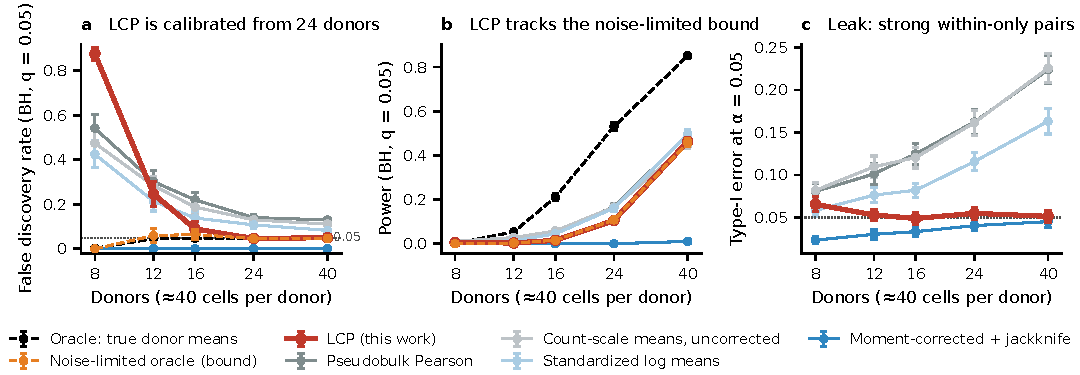
\includegraphics[width=\textwidth]{figures/fig_sim.pdf}
\caption{Development simulations ($R=200$ replicates per point; bars $\pm2$ MCSE; $\sim$40 cells per donor). (a) BH false discovery rate. (b) BH power. (c) Type-I error at $\alpha=0.05$ for strong within-only pairs ($\SB_{jk}=0$, $\SW_{jk}>0$), the pairs that leak into donor means. ORACLE uses the true donor means; BOUND adds noise of the true sampling variance without leak (the noise-limited benchmark of Theorem~\ref{thm:bound}).}\label{fig:sim}\end{figure}
\paragraph{Results.} Table~\ref{tab:sim} and Fig.~\ref{fig:sim} summarize. \emph{From 24 donors}, LCP controls the FDR (\LCPFDRDtwentyfour{} at $D=24$, \LCPFDRDforty{} at $D=40$) and its power equals BOUND's (\LCPpowDtwentyfour{} vs \BOUNDpowDtwentyfour{}; \LCPpowDforty{} vs \BOUNDpowDforty{}); MC is valid but nearly powerless (\MCpowDforty{} at $D=40$); PB, E5 and naive have slightly higher nominal power but inflated FDR (PB \PBFDRrange{}; E5 and naive \OtherFDRrange{}), driven by within-only pairs (type-I error up to \PBSSmax{} for the strong within-only program). The ORACLE's much higher power (\ORACLEpowDforty{} at $D=40$) is the price of measurement noise predicted by Theorem~\ref{thm:bound}, not a deficiency of the test: LCP's power equals BOUND's in every design, although below 24 donors that power comes with an inflated FDR. \emph{At 16 or fewer donors}, every method that uses observed donor means is anti-conservative in the tail: LCP's FDR is \LCPFDRDsixteen{} at $D=16$, \LCPFDRDtwelve{} at $D=12$ and \LCPFDRDeight{} at $D=8$, while BOUND and ORACLE stay near 0.05. The excess comes mostly from independent pairs. A plausible mechanism is that donors with few cells have heavy-tailed noise in both genes at once, which the identity pairing multiplies and random pairings dilute; standardization equalizes variances but not tails. Held-out results (Table~\ref{tab:heldout}, Appendix) \HELDOUTsentence

\paragraph{Intervals: a negative result.} For linear-scale $\SB_{jk}$, 95\% intervals undercover under skewed donor effects at every donor number we examined, \emph{including intervals computed from the true donor means}: normal-theory oracle intervals cover 0.85--0.88 for between-donor pairs at 16 to 84 donors, and donor bootstrap-$t$ oracle intervals 0.86--0.95. Our deployed bootstrap-$t$ interval tracks the oracle but falls more than 0.02 below it in 15 of 60 class--design cells. We therefore claim calibrated tests, not calibrated intervals.

\section{Real data: microglia from two Alzheimer's disease cohorts}
\begin{figure}[t]\centering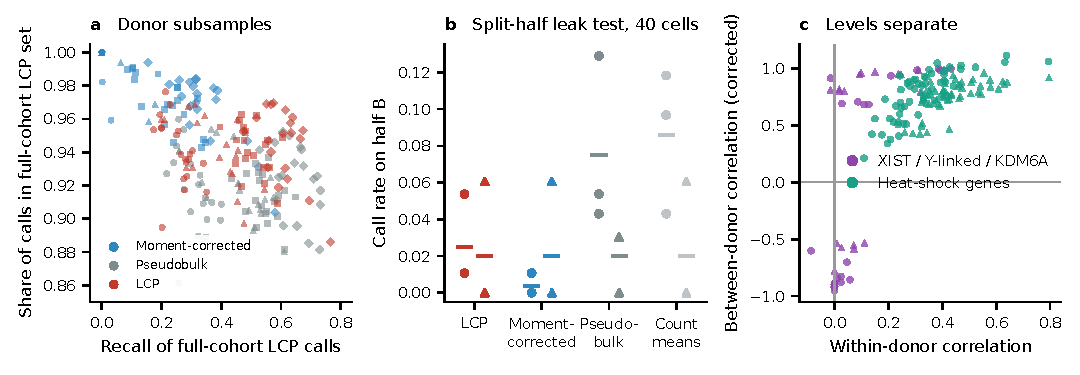
\includegraphics[width=\textwidth]{figures/fig_real.pdf}
\caption{Real data. (a) Twenty random 24- or 40-donor subsets per cohort; precision and recall of each method's calls against the full-cohort LCP calls (an estimate, not truth). Circles, SEA-AD 24; squares, SEA-AD 40; triangles, Lee 24; diamonds, Lee 40. (b) Call rate at 40 cells per donor among the top-1\% within-donor co-expressed pairs that show no between-donor evidence in the full cohort (three random cell draws per cohort; circles SEA-AD, triangles Lee; bars are means). (c) Corrected between-donor versus within-donor correlation for sex-linked and heat-shock gene pairs in both cohorts (circles SEA-AD, triangles Lee).}\label{fig:real}\end{figure}
\paragraph{Data.} We used two public CELLxGENE cohorts: SEA-AD middle temporal gyrus microglia/PVM (10x 3$'$ v3 nuclei only; 84 donors; 34{,}794 nuclei; 18--1{,}068 per donor) \citep{Gabitto2024SEAAD} and Lee et al.\ 2026 fresh prefrontal-cortex microglia \citep{Lee2026}. For Lee we used a subset fixed before this study to keep the file tractable: 80 donors drawn at random, stratified by disease status, from the donors with at least 1{,}600 microglia, and 1{,}600 random cells from each (seed 20261022). Lee is therefore a high-reliability contrast to SEA-AD and over-represents donors with many cells. We analysed \RealG{} genes: the 400 most expressed in both cohorts and 17 further heat-shock, sex-linked and perivascular-macrophage control genes (\RealPairs{} pairs), with identical gene order across cohorts. LCP used $4\times10^5$ permutations on the full cohorts and $10^5$ elsewhere, for all pairs, on GPUs (about 15\,s per full cohort).

\paragraph{Between-donor co-expression calls are common.} With all donors, LCP calls \SEAADfullLCP{} (SEA-AD) and \LEEfullLCP{} (Lee) pairs at FDR 0.05, a fraction of \SEAADfullLCPfrac{} and \LEEfullLCPfrac{} of all pairs; pseudobulk calls \SEAADfullPB{} and \LEEfullPB{}, and the moment-corrected test \SEAADfullMC{} and \LEEfullMC{}. The per-pair reliabilities give $\Deff/D$ medians of \DeffSEAADfull{} and \DeffLEEfull{} at the cohorts' real cell numbers, but only \DeffSEAADcap{} and \DeffLEEcap{} when each donor is reduced to 40 cells (Theorem~\ref{thm:bound}). Sex-linked pairs are a positive control for a purely between-donor association: \emph{XIST} versus Y-linked genes have corrected between-donor correlations of \sexRhoRange{} with within-donor correlations of at most \sexWithinMax{} in absolute value. Heat-shock genes co-vary at both levels (median between-donor correlation \hsRhoSEAAD{} in SEA-AD and \hsRhoLEE{} in Lee; within-donor \hsWSEAAD{} and \hsWLEE{}).

\paragraph{The leak in real data.} At the cohorts' real depths the estimated leak is a small part of the pseudobulk covariance: over the pairs that pseudobulk calls, the median ratio of the estimated leak $D^{-1}\sum_d\kappa_d\hat C_{d,jk}$ to the count-scale covariance of donor means is \SEAADleakFull{} in SEA-AD and \LEEleakFull{} in Lee. This is consistent with Lemma~\ref{lem:leak}, because hundreds of cells per donor make $\bar\kappa$ small. The pairs pseudobulk calls are dominated by strong between-donor associations, however; for pairs that co-vary only within donors the leak is, by definition, the whole signal. To see the leak without reusing cells, we split each donor's cells at random into halves A and B. Half A selected within-donor-only pairs: the top 1\% by within-donor correlation that showed no between-donor evidence (LCP and pseudobulk $p>0.05$; \capNwithin{} pairs). Half B, reduced to 40 cells per donor (three random draws; donors with fewer cells kept all of them), was used only for testing. There the median leak share among pseudobulk calls rises to \SEAADleakSplit{} (SEA-AD) and \LEEleakSplit{} (Lee). In SEA-AD, pseudobulk calls \capPBSEAAD{} of the within-only pairs, uncorrected count-scale means \capnaiveSEAAD{} and LCP \capLCPSEAAD{}; in Lee all methods call \capLCPLEE{}. These counts are small, so the rates are imprecise.

\paragraph{Stability under donor subsampling.} We drew 20 random subsets of 24 and of 40 donors from each cohort and compared their calls with the full-cohort LCP calls, which are themselves estimates. At 24 donors, the fraction of calls that are full-cohort calls of the same sign was \precLCPDtwentyfour{} for LCP, \precPBDtwentyfour{} for pseudobulk and \precMCDtwentyfour{} for the moment-corrected test, which recovered \recMCDtwentyfour{} of the full-cohort calls against \recLCPDtwentyfour{} for LCP. At 40 donors: precision \precLCPDforty{}, \precPBDforty{} and \precMCDforty{}; recall \recLCPDforty{}, \recPBDforty{} and \recMCDforty{}. Because the reference is LCP's own full-cohort call set, this comparison favours LCP and measures stability, not accuracy; the clear finding is that the moment-corrected test recovers few pairs at these donor numbers.

\paragraph{Replication across cohorts.} Of SEA-AD LCP calls, \replLCP{} are LCP calls of the same sign in Lee (pseudobulk: \replPB{}); the rank correlation of pair statistics across cohorts is \rhoLCP{} for LCP and \rhoPB{} for pseudobulk. Crossing the methods gives the same picture: SEA-AD LCP calls are replicated by Lee pseudobulk calls at \xLCPbyPB{}, and SEA-AD pseudobulk calls by Lee LCP calls at \xPBbyLCP{}. The \nPBonly{} pairs called by pseudobulk but not by LCP in SEA-AD replicate as LCP calls in Lee at \replPBonly{}. They are borderline pairs, though, so this lower rate is not by itself evidence of leak. At these cell numbers the leak is small, and the two methods give similar results; the difference matters when donors contribute tens of cells.

\paragraph{Checking the assumptions (post hoc).} Two features of the real data qualify these results. First, depth is not independent of cell state. The pooled within-donor correlation between log library size and a gene's library-normalized count, which is zero in expectation under Lemma~\ref{lem:leak}'s assumption, has median \cplMedSEAAD{} in SEA-AD (median absolute value \cplAbsSEAAD{}) and \cplMedLEE{} in Lee (\cplAbsLEE{}). Its absolute value exceeds \cplStressW{}, the median for the coupled genes of the stress design, for \cplFracSSEAAD{} and \cplFracSLEE{} of the genes, and exceeds 0.1 for \cplFracTSEAAD{} and \cplFracTLEE{}. The within-donor spread of log library size (\sdLibSEAAD{}, \sdLibLEE{}) matches the simulated null (\sdLibNull{}) rather than the stress design (\sdLibStress{}), so the real data are not a replica of the stress design. They do show that depth--state coupling of that size is common, and LCP's stress-design FDR of \STRESSLCPFDR{} applies to the real-data calls as a warning. Second, the donor means have a strong low-rank structure: the first principal component of the standardized donor means carries \pcOneSEAAD{} (SEA-AD) and \pcOneLEE{} (Lee) of their variance, against at most \pcNullSEAAD{} and \pcNullLEE{} after permuting each gene across donors. It is not explained by mean library size, cell number, sex or (SEA-AD) mitochondrial fraction ($|r|\le\pcCorrMaxSEAAD{}$ and $\le\pcCorrMaxLEE{}$). A shared donor factor, biological or technical, is the likely reason that LCP calls \SEAADfullLCPfrac{}--\LEEfullLCPfrac{} of all pairs; adjusting for it changes the estimand and is left for future work.


\section{Discussion}

Between-donor co-expression is a different estimand from within-donor co-expression, and pseudobulk correlation does not estimate it: it adds $\bar\kappa\SW$, a leak that grows as cells per donor shrink. The leak is removable, and LCP removes it while remaining calibrated from about two dozen donors, at the power of a noise-limited oracle. Theorem~\ref{thm:bound} makes explicit what no method can recover: with ${\sim}40$ cells per donor, $D$ donors carry the per-pair information of about $D/3$ perfectly measured donors, so 16-donor rare-cell studies cannot resolve pair-level between-donor structure, and adding donors helps far more than sequencing more cells. Below 24 donors our test is not reliable in the tail, nor is any competitor we examined that uses observed donor means; covariance intervals undercover there even with true donor means.

\paragraph{Limitations.} The analysis assumes Poisson counts given latent expression, depth independent of cell state within donors, and independent donors; violations of the second (depth--state coupling) are evaluated as a stress design. LCP tests independence of donor effects, not zero covariance. Gene-level borrowing across programs (e.g.\ low-rank between-donor models) could exceed the per-pair bound but changes the estimand and is left for future work. Real-data reference calls are themselves estimates.

\paragraph{Code and data.} Code, pre-registrations, frozen specifications and scripts for every figure: \url{https://github.com/kaapra081/fewdonor-coexpression}. Data are public CELLxGENE datasets (SEA-AD MTG microglia c76098ba-eed3-45b1-98f2-96fcac55ed18; Lee et al.\ 2026 fresh myeloid 440da0a0-f321-4f40-9080-bb04031681e5); the repository contains a download script with dataset version identifiers and checksums.

\bibliographystyle{unsrtnat}
\bibliography{refs}

\clearpage
\appendix
\section{Proofs}\label{app:proofs}

\paragraph{Proof of Lemma~\ref{lem:leak}.}
Condition on $F_d$ and the design. Since $\mathrm{E}[x_{ij}\mid\theta_i,s_i]=\theta_{ij}$, $\mathrm{E}[m_{dj}]=\sum_is_i\mu_{dj}/S_d=\mu_{dj}$. For $j\neq k$ the Poisson draws are independent given $\theta_i$, so $\mathrm{Cov}(x_{ij},x_{ik}\mid\theta_i,s_i)=0$ and $\mathrm{Cov}(x_{ij},x_{ik})=\mathrm{Cov}_{F_d}(\theta_j,\theta_k)$; cells are independent, hence $\mathrm{Cov}(m_{dj},m_{dk})=\sum_is_i^2\mathrm{Cov}_{F_d}(\theta_j,\theta_k)/S_d^2$. The law of total covariance over $F_d$ gives $\mathrm{Cov}(m_{dj},m_{dk})=\mathrm{Cov}(\mu_{dj},\mu_{dk})+\kappa_d\,\mathrm{E}[\mathrm{Cov}_{F_d}(\theta_j,\theta_k)]=\SB_{jk}+\kappa_d\SW_{jk}$. Finally $\hat C_{d,jk}$ is the unbiased sample covariance of $n_d$ i.i.d.\ vectors $x_i$ whose off-diagonal covariance is $\mathrm{Cov}_{F_d}(\theta_j,\theta_k)$. \qed

\begin{proposition}[Unbiased weighted estimator]\label{prop:unbiased}
For fixed centring weights $\alpha,\beta$ with $\sum_d\alpha_d=\sum_d\beta_d=1$ and fixed weights $w_d$, let $r_{dj}=m_{dj}-\sum_e\alpha_em_{ej}$, $r_{dk}=m_{dk}-\sum_e\beta_em_{ek}$, $\hat\ell_d=\kappa_d\hat C_{d,jk}$ and $A=\sum_e\alpha_e\beta_e$. Then
\[\hat\SB(w)=\frac{\sum_dw_d\big[r_{dj}r_{dk}-\hat\ell_d(1-\alpha_d-\beta_d)-\sum_e\alpha_e\beta_e\hat\ell_e\big]}{\sum_dw_d(1-\alpha_d-\beta_d+A)}\]
is unbiased for $\SB_{jk}$; with $w\equiv1$ and $\alpha=\beta=1/D$ it equals $S_{B,jk}-D^{-1}\sum_d\hat\ell_d$.
\end{proposition}
\begin{proof}
Let $c_d=\mathrm{Cov}(m_{dj},m_{dk})=\SB_{jk}+\lambda_d$ with $\lambda_d=\kappa_d\SW_{jk}$. Independence across donors gives $\mathrm{E}[r_{dj}r_{dk}]=c_d(1-\alpha_d-\beta_d)+\sum_e\alpha_e\beta_ec_e$. Substituting $c_d$ and $\mathrm{E}\hat\ell_d=\lambda_d$, the $\lambda$ terms cancel and the numerator has expectation $\SB_{jk}\sum_dw_d(1-\alpha_d-\beta_d+A)$.
\end{proof}

\paragraph{Proof of Theorem~\ref{thm:bound}.}
For a bivariate normal with covariance $V=\begin{psmallmatrix}a&c\\c&b\end{psmallmatrix}$, $\partial V/\partial c=E=\begin{psmallmatrix}0&1\\1&0\end{psmallmatrix}$ and the Fisher information is $I_{cc}=\tfrac12\mathrm{tr}(V^{-1}EV^{-1}E)$. With $\Delta=ab-c^2$, $V^{-1}E=\Delta^{-1}\begin{psmallmatrix}-c&b\\a&-c\end{psmallmatrix}$ and $\mathrm{tr}\{(V^{-1}E)^2\}=2(ab+c^2)/\Delta^2$, which gives $I_d$. For $E_a=\partial V/\partial a$, $\tfrac12\mathrm{tr}(V^{-1}EV^{-1}E_a)=-bc/\Delta^2$, which vanishes at $c=0$ (likewise for $b$), and mean parameters are orthogonal to covariance parameters in the normal family; the efficient information at $\sigma=0$, $\ell\equiv0$ is therefore $\sum_d1/(a_db_d)$. The oracle observes $\mu_d$, i.e.\ $\psi\equiv0$, giving $I^\ast=D/(\SB_{jj}\SB_{kk})$. The model is locally asymptotically normal in $\sigma$ with these informations, and the Neyman--Pearson bound for local alternatives $h/\sqrt D$ in the limiting Gaussian shift experiment \citep[ch.~15]{vanderVaart1998} implies that no asymptotically level-$\alpha$ test exceeds power $1-\Phi(z_{\alpha/2}-|h|\bar I^{1/2})+\Phi(-z_{\alpha/2}-|h|\bar I^{1/2})$ with $\bar I=\lim D^{-1}I$. The oracle with $D'$ donors attains this when $D'/(\SB_{jj}\SB_{kk})=\sum_d1/(a_db_d)$, i.e.\ $D'=\sum_d\rho_{dj}\rho_{dk}$. \qed

\paragraph{Proof of Theorem~\ref{thm:lcp}.}
(a) Under $H_0$ with no leak, the standardized vectors $r_{\cdot j}$ and $r_{\cdot k}$ are functions of disjoint, independent data (each gene's nuisance estimates use only that gene), hence independent; if $r_{\cdot j}$ is exchangeable, $(r_{\pi(\cdot)j},r_{\cdot k})$ has the same law as $(r_{\cdot j},r_{\cdot k})$ for every $\pi$, and the randomization $p$-value is valid by the standard argument. (b) \emph{Outline.} Replace estimated by true nuisance parameters; the difference is $O_p(D^{-1/2})$ in $T/\sqrt D$. Under $H_0$, by Lemma~\ref{lem:leak}, $\mathrm{E}[r_{dj}r_{dk}]=\ell_d/(v_{dj}v_{dk})^{1/2}$, so the summands $r_{dj}r_{dk}-\tilde\ell_d$ are independent with mean zero and variance $1+\tilde\ell_d^2+\gamma_d$, where $\gamma_d$ is a fourth-cumulant term of the within-donor sampling error of order $1/n_d$ (zero under Gaussian sampling error). Lyapunov's central limit theorem and the $\sqrt{D/(D+\sum\tilde\ell^2)}$ scaling give $T/\sqrt D\Rightarrow N(0,1)$. For the permutation distribution, $\sum_dr_{dj}^2=D-1$ by the Paule--Mandel estimating equation and $\max_dr_{dj}^2/D\to0$ in probability, so Hoeffding's combinatorial central limit theorem \citep{Hoeffding1951} gives $T^\pi/\sqrt D\Rightarrow N(0,1)$ conditionally. The finite-$D$ accuracy of these approximations in the BH-relevant tail is what Section~6 measures; it fails below about 24 donors.

\paragraph{Proof of Proposition~\ref{prop:are} (outline).}
Under the Gaussian model with local alternative $\sigma=h/\sqrt D$, $\mathrm{E}[r_{dj}r_{dk}-\tilde\ell_d]=\sigma/(a_db_d)^{1/2}=\sigma(\rho_{dj}\rho_{dk})^{1/2}/(\SB_{jj}\SB_{kk})^{1/2}$ and the null variance per donor is $1+O(\ell^2)$, so the noncentrality of $T/\sqrt D$ is $h\,D^{-1}\sum_d(\rho_{dj}\rho_{dk})^{1/2}/(\SB_{jj}\SB_{kk})^{1/2}$. Squaring and dividing by the efficient information $\bar I$ gives the stated ratio; Cauchy--Schwarz gives $\le1$.

\section{Pre-registration and changes}\label{app:prereg}
Development gates, code hashes and the held-out specification were written and hashed before the corresponding runs and pushed to the repository (commits d00b9c2, eee7366, c986bab). Two development criteria were amended before the affected results were inspected, with reasons: (1) the usefulness criterion was changed from ``half the ORACLE's power at 16 donors'' to ``at least 80\% of BOUND's power'' after exploratory runs showed, and Theorem~\ref{thm:bound} implies, that no per-pair test can approach the ORACLE at 16 donors with ${\sim}40$ cells; (2) the interval criterion was changed to ``within 0.02 of the oracle interval'' after exploratory runs showed that oracle intervals themselves undercover. Under the original criteria, and under the amended interval criterion, the method fails at $D\le16$; we report this in the main text. Development seeds, held-out seeds, panel seeds and designs are listed in the repository.

\section{Additional tables}\begin{table}[t]\centering\footnotesize\setlength{\tabcolsep}{2.5pt}
\caption{Development simulations ($R=200$ per design; panel of 3{,}160 pairs). BH at $q=0.05$; MCSE of FDR $\le$0.031 and of power $\le$0.011 throughout (full values in the repository).}\label{tab:simfull}
\begin{tabular}{lcccccccccccccc}
\toprule
& \multicolumn{2}{c}{LCP} & \multicolumn{2}{c}{BOUND} & \multicolumn{2}{c}{ORACLE} & \multicolumn{2}{c}{PB} & \multicolumn{2}{c}{E5} & \multicolumn{2}{c}{naive} & \multicolumn{2}{c}{MC} \\
Design & FDR & Pow & FDR & Pow & FDR & Pow & FDR & Pow & FDR & Pow & FDR & Pow & FDR & Pow \\
\midrule
8 & 0.876 & 0.005 & 0.000 & 0.000 & 0.003 & 0.000 & 0.541 & 0.006 & 0.424 & 0.006 & 0.475 & 0.011 & 0.000 & 0.000 \\
12 & 0.246 & 0.003 & 0.059 & 0.003 & 0.045 & 0.054 & 0.301 & 0.016 & 0.214 & 0.013 & 0.283 & 0.028 & 0.000 & 0.000 \\
16 & 0.089 & 0.015 & 0.065 & 0.016 & 0.047 & 0.210 & 0.220 & 0.047 & 0.138 & 0.045 & 0.188 & 0.058 & 0.000 & 0.000 \\
24 & 0.046 & 0.105 & 0.046 & 0.108 & 0.047 & 0.531 & 0.140 & 0.168 & 0.108 & 0.161 & 0.130 & 0.166 & 0.000 & 0.000 \\
40 & 0.050 & 0.463 & 0.048 & 0.458 & 0.051 & 0.851 & 0.129 & 0.494 & 0.083 & 0.497 & 0.111 & 0.449 & 0.000 & 0.010 \\
16, strong & 0.065 & 0.187 & 0.049 & 0.186 & 0.048 & 0.578 & 0.138 & 0.321 & 0.092 & 0.291 & 0.135 & 0.297 & 0.000 & 0.000 \\
16, stress$^\dagger$ & 0.224 & 0.012 & 0.045 & 0.008 & 0.047 & 0.230 & 0.247 & 0.035 & 0.159 & 0.041 & 0.302 & 0.050 & 0.000 & 0.000 \\
\bottomrule
\end{tabular}
\end{table}

\begin{table}[t]\centering\caption{Held-out evaluation pending.}\label{tab:heldout}\end{table}



\end{document}
